
\documentclass[10pt,a4]{article}
\usepackage[english]{babel}
\usepackage[utf8x]{inputenc}
\usepackage{amsmath}
\usepackage{graphicx}
\usepackage[colorinlistoftodos]{todonotes}
\usepackage{blindtext}
\usepackage{geometry}
\geometry{top=3cm,left=2cm,right=2cm,bottom=3cm}
\usepackage[scaled]{helvet}
\usepackage[T1]{fontenc}
\usepackage{url}
\renewcommand\familydefault{\sfdefault}
\usepackage{wrapfig} % wrap text around figures
\usepackage[section]{placeins}



\usepackage{listings} % code
\usepackage{xcolor} % colors for synthax highlight
\usepackage{url} % cite urls in bib
\usepackage{float} % prevent image repositioning

% Custom commands
\newcommand{\stm}{\texttt{STM32F411 }}
\newcommand{\ws}{\texttt{WS2812 }}
\newcommand{\spi}{\texttt{SPI }}
\newcommand{\type}{\char`_t}
\newcommand{\dma}{\texttt{DMA }}
\newcommand{\nucleo}{\texttt{Nucleo }}

\lstset { % for code
    language=C++,
    breaklines=true,
     basicstyle=\color{teal}
}

\author{Valerio Nappi}
\date{\today}
\title{A WS2812 smart LED driver for Miosix}



\begin{document}
\maketitle
\tableofcontents

\begin{center}
NOTE: IT IS MANDATORY TO FILL IN ALL THE SECTIONS AND SUBSECTIONS IN THIS TEMPLATE
\end{center}

\section{Project data}

\begin{itemize}
\item 
  Project supervisor(s): Federico Terraneo

\item 
Describe in this table the group that is delivering this project:

\begin{center}
\begin{tabular}{lll}
Last and first name & Person code & Email address\\
\hline
  Valerio Nappi & NOPENOPENOPE & NOPENOPENOPE@NOPENOPENOPE.it
\end{tabular}
\end{center}

\item
Describe here how development tasks have been subdivided among members
of the group, e.g.:

\begin{itemize}
\item The work was entirely conducted by the only author
\end{itemize}

\item Links to the project source code; Put here, if available, links to public repos hosting your project 
\item https://github.com/valerionew/WS2812-driver and https://github.com/valerionew/miosix-kernel

\end{itemize}


\section{Project description}
The scope of this project is to create a C++ driver for Miosix for the \ws addressable LEDs. In particular, the \spi peripheral will be exploited to generate the data stream for the LEDs. The driver will be independent of the particular platform or framework. The aim of this project is to achieve a high FPS refresh update for the LEDs, and the target is set at 30 FPS on an \stm microcontroller

\subsection{\ws LEDs}
The \ws smart LEDs are designed to be connected in a daisy-chain, where each smart LED passes to the next smart LED all the packets received, but the first it receives.
The packets are 24 bits long and are structured as 8-bit green, 8-bit red, 8-bit blue (in GRB order).

\begin{figure}[H]
\centering
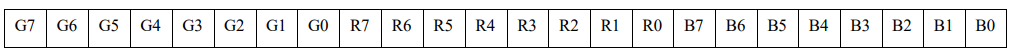
\includegraphics[width=\linewidth]{grb.png}
\caption{\label{fig:grb}The bit ordering for the \ws LEDs}
\end{figure}
 

\begin{wrapfigure}[11]{r}{0.25\textwidth}
\centering
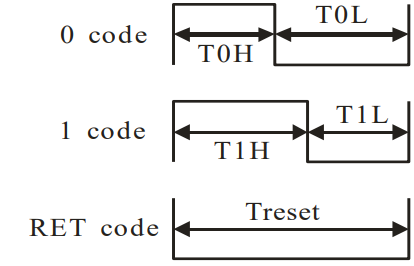
\includegraphics[width=\linewidth]{encoding.png}
\caption{\label{fig:encoding}The encoding for the \ws LEDs}
\end{wrapfigure}

The bits are encoded with a specific encoding, with a fixed period for each bit and variable duty to signal '0' and '1'.
The data is shown when each led does not receive an input (D = '0') for a fixed amount of time. This is called RESET time.

The aim of this project is to use the \spi peripheral of an \stm micro-controller to generate the data-stream for the LED. This is done by varying the ratio of '0's and '1's  to represent each bit.
The easiest case is to use the correspondence \texttt{1 bit : 8 bits}, notice that this approach requires $24+3 \text{ bytes}$ of memory for each LED. However, the number of bits-per-bit, does not influence the refresh rate, as the timing per symbol is fixed. 

\begin{wraptable}[9]{r}{0.5\textwidth}
\begin{tabular}{|c|c|c|c|}
\hline
sym & description & time & tolerance \\
\hline
T0H & '0'  code, high voltage time & 0.4us &±150ns \\
T1H & '1'  code, high voltage time & 0.8us &±150ns \\
T0L & '0'  code, low voltage time  & 0.85us& ±150ns \\
T1L & '1'  code, low voltage time  & 0.45us &±150ns\\
RES & low voltage time & Above 50µs& \\
TH+TL & total period time & 1.25us & ±600ns \\
\hline
\end{tabular}
\caption{\label{tab:timings}Timings for the \ws protocol}
\end{wraptable}
\FloatBarrier % does not work
\subsection{Timing requirements}

% i hate you latex
%\begin{wrapfigure}[9]{r}{0.57\textwidth}
% 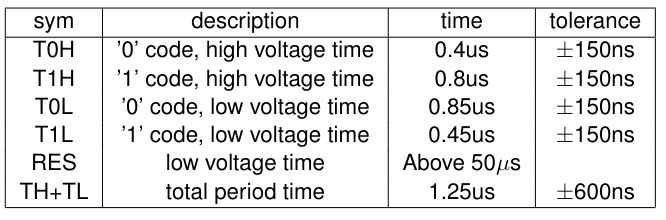
\includegraphics[width=\linewidth]{WStimings.png}
%\caption{\label{fig:timings}Timings for the \ws protocol}
%\end{wrapfigure}


Timing requirements for this protocol are quite relaxed, and field tests \cite{cpldcpu} have proven them even more relaxed. Considering the \texttt{1 bit : 8 bits} correspondence, the total byte time should be at least 650ns and at most 1.85us. This leads to \spi speeds between 12.30 Mbit/s and 4.32 Mbit/s, nominally it should be 6.40 Mbit/s. 
For our implementation we set the \spi speed at 9.0 Mbit/s as it is easy to configure the clocks to obtain it, without affecting the system clock. Our symbols of choice are, for '0' \texttt{0b11000000}, and for '1' \texttt{0b11111100}.

\subsection{Design and implementation}
\subsubsection{Class design}
Two classes are implemented for this project:
\begin{itemize}
    \item 
the \lstinline{RGB_t<typename T>} class, that is a template class that represents the triplet of RGB of an arbitrary type, in our case \texttt{uint8\type};
    \item the \lstinline{WS2812<int LENGTH>} class, which is responsible for the driving of the LEDs, the creation of the \spi buffer and the call of an user-supplied \spi call.
    \item is an additional header providing already defined \lstinline{RGB_t<uint8_t>}colors
\end{itemize}

The user has to set the \spi to the correct speed and hand over the \spi function to do the write. The so-composed class is already compatible with the DMA, as the driver is agnostic on how the \spi function works. This also makes the class cross-platform compatible, as long as a \lstinline{spi_transfer(uint8_t* data, uint16_t length)} is provided to it.

\subsubsection{Thread synchronization}


Two threads are implemented on Miosix for this project:
\begin{itemize}
\item The main thread, that writes the frame in the frame-buffer;
\item The consumer thread, that sets up the \dma controller to read the frame-buffer and output the bytes via the \spi peripheral.
\end{itemize}
It is clear how there is  concurrency between these threads on the frame-buffer. The access to the frame-buffer is regulated with a \textbf{thread synchronization} mechanism. The main thread warns the consumer thread that the data is ready using the \lstinline{full} \textbf{condition variable}. The \lstinline{Thread},  \lstinline{Mutex} and  \lstinline{ConditionVariable} classes are native to Miosix and readilty available.   \\

This \textbf{mutex} and \textbf{condition variable} paradigm allows for \textbf{thread-safe} access of the shared resources. This approach renders also efficient the execution of the consumer thread, that remains on hold up until when new data is available to write on the peripheral and the \lstinline{full} condition variable is signaled. The main thread is put to sleep for $\tau = 1 /\text{frame-rate}$. \\

The \textbf{lock} on the mutex is acquired by the thread according to the \textbf{RAII} paradigm. This \texttt{C++} paradigm is very common in this context, where the lock is instantiated in a scope and gets destroyed at the end of it. The advantage of this technique is that it prevents errors such as forgetting to release the lock when exiting the critical section. The lock is also considered released if the execution of the holder is, for any reason, disrupted.\\

The same technique is used to prevent interrupts from disrupting some operations that shall be \textbf{atomic}, such as the setup of the \texttt{RCC} (Reset and Clock Control) unit, that may be accessed by multiple peripherals concurrently. By acquiring a lock on the interrupts with \lstinline{FastInterruptDisableLock Lock}, the interrupts are disabled until the object is destroyed.


\subsubsection{DMA and interrupt handling}
The \dma implementation does also exploit some \textbf{interrupts} to warn the software that the hardware \dma has completed the transmission. With this mechanism it is possible to release the lock on the shared buffer only on completion.\\

The interrupt handling on it's own requires some operating systems mechanisms. After clearing possible previous interrupts and enabling the interrupts for the \texttt{DMA}, the \dma is set, the process is placed in a \textbf{wait queue} and the control is yielded back to the \textbf{scheduler}. When the interrupt arrives, after reading possible errors and clearing the interrupt flag, the interrupt handler compares the current thread priority with the priority of the consumer. If the waiting thread has higher priority, it is scheduled right away. Otherwise the interrupt handler just returns, and the consumer thread will be resumed when it's time.\\

Clearing the \textbf{interrupt} flag is done by simply writing \texttt{1} in the Flag Clear Register of the \dma peripheral, in contrast with the clear by writing \texttt{0/1}, that is used in registers that can be written both by the hardware and by the software.

\clearpage

\section{Project outcomes}

\subsection{Concrete outcomes}
The main demo for this project is composed by a \texttt{NUCLEO-F411} development board with a strip of 60 \ws LEDs. The demo can update the LED animation at more than 300 FPS, far exceeding the required frame-rate. With this amount of spare resources available, it would be fairly easy to stay above the 30 FPS mark for as much as 600 \ws LEDs.

\begin{wrapfigure}[11]{r}{0.4\textwidth}
\includegraphics[width=\linewidth]{example-image-a}
\caption{\label{fig:encoding}The demo for the project}
\end{wrapfigure}
\subsection{Learning outcomes}

This project was very useful to learn and apply all the  techniques and paradigms seen in the course, especially in an embedded context. It also taught the author how to approach a new code base, and how to debug in it.

Examples:


\subsection{Existing knowledge}
The Sensor System course was helpful for this project, as it taught the basics of STM32 HAL development, which were very useful in the first stage of the project, where the \ws Class was being tested in a known environment. A spare time read, \cite{kormanyos2021real}, was also helpful in mastering the \texttt{C++} concepts from an embedded point of view.


\subsection{Problems encountered}
The two biggest problems encountered while developing this project were:
\begin{itemize}
\item Short time available: this project was developed due to the need to change from the previous project. The project was therefore developed in a handful of weeks.
\item Non-functioning UART on the \stm \texttt{Nucleo}: the UART was not functioning on the target board. 
\end{itemize}

\section{Honor Pledge}
(\textbf{This part cannot be modified and it is mandatory to sign it})

I/We pledge that this work was fully and wholly completed within the criteria
established for academic integrity by Politecnico di Milano (Code of Ethics and
Conduct) and represents my/our original production, unless otherwise cited.

I/We also understand that this project, if successfully graded,  will fulfill part B requirement of the
Advanced Operating System course and that it will be considered valid up until
the AOS exam of Sept. 2022. 

\begin{flushright}
Group Students' signatures
\end{flushright}

\bibliographystyle{alpha}
\bibliography{sample}

\end{document}
